\begin{appendices}
\addtocontents{toc}{\protect\setcounter{tocdepth}{2}}\makeatletter
\addtocontents{toc}{%
  \begingroup
  \let\protect\l@chapter\protect\l@section
  \let\protect\l@section\protect\l@subsection
}
\makeatother


\section{General deployment diagram}\label{app:deployment-diagram}
\begin{landscape}
   \begin{figure}
    \centering
    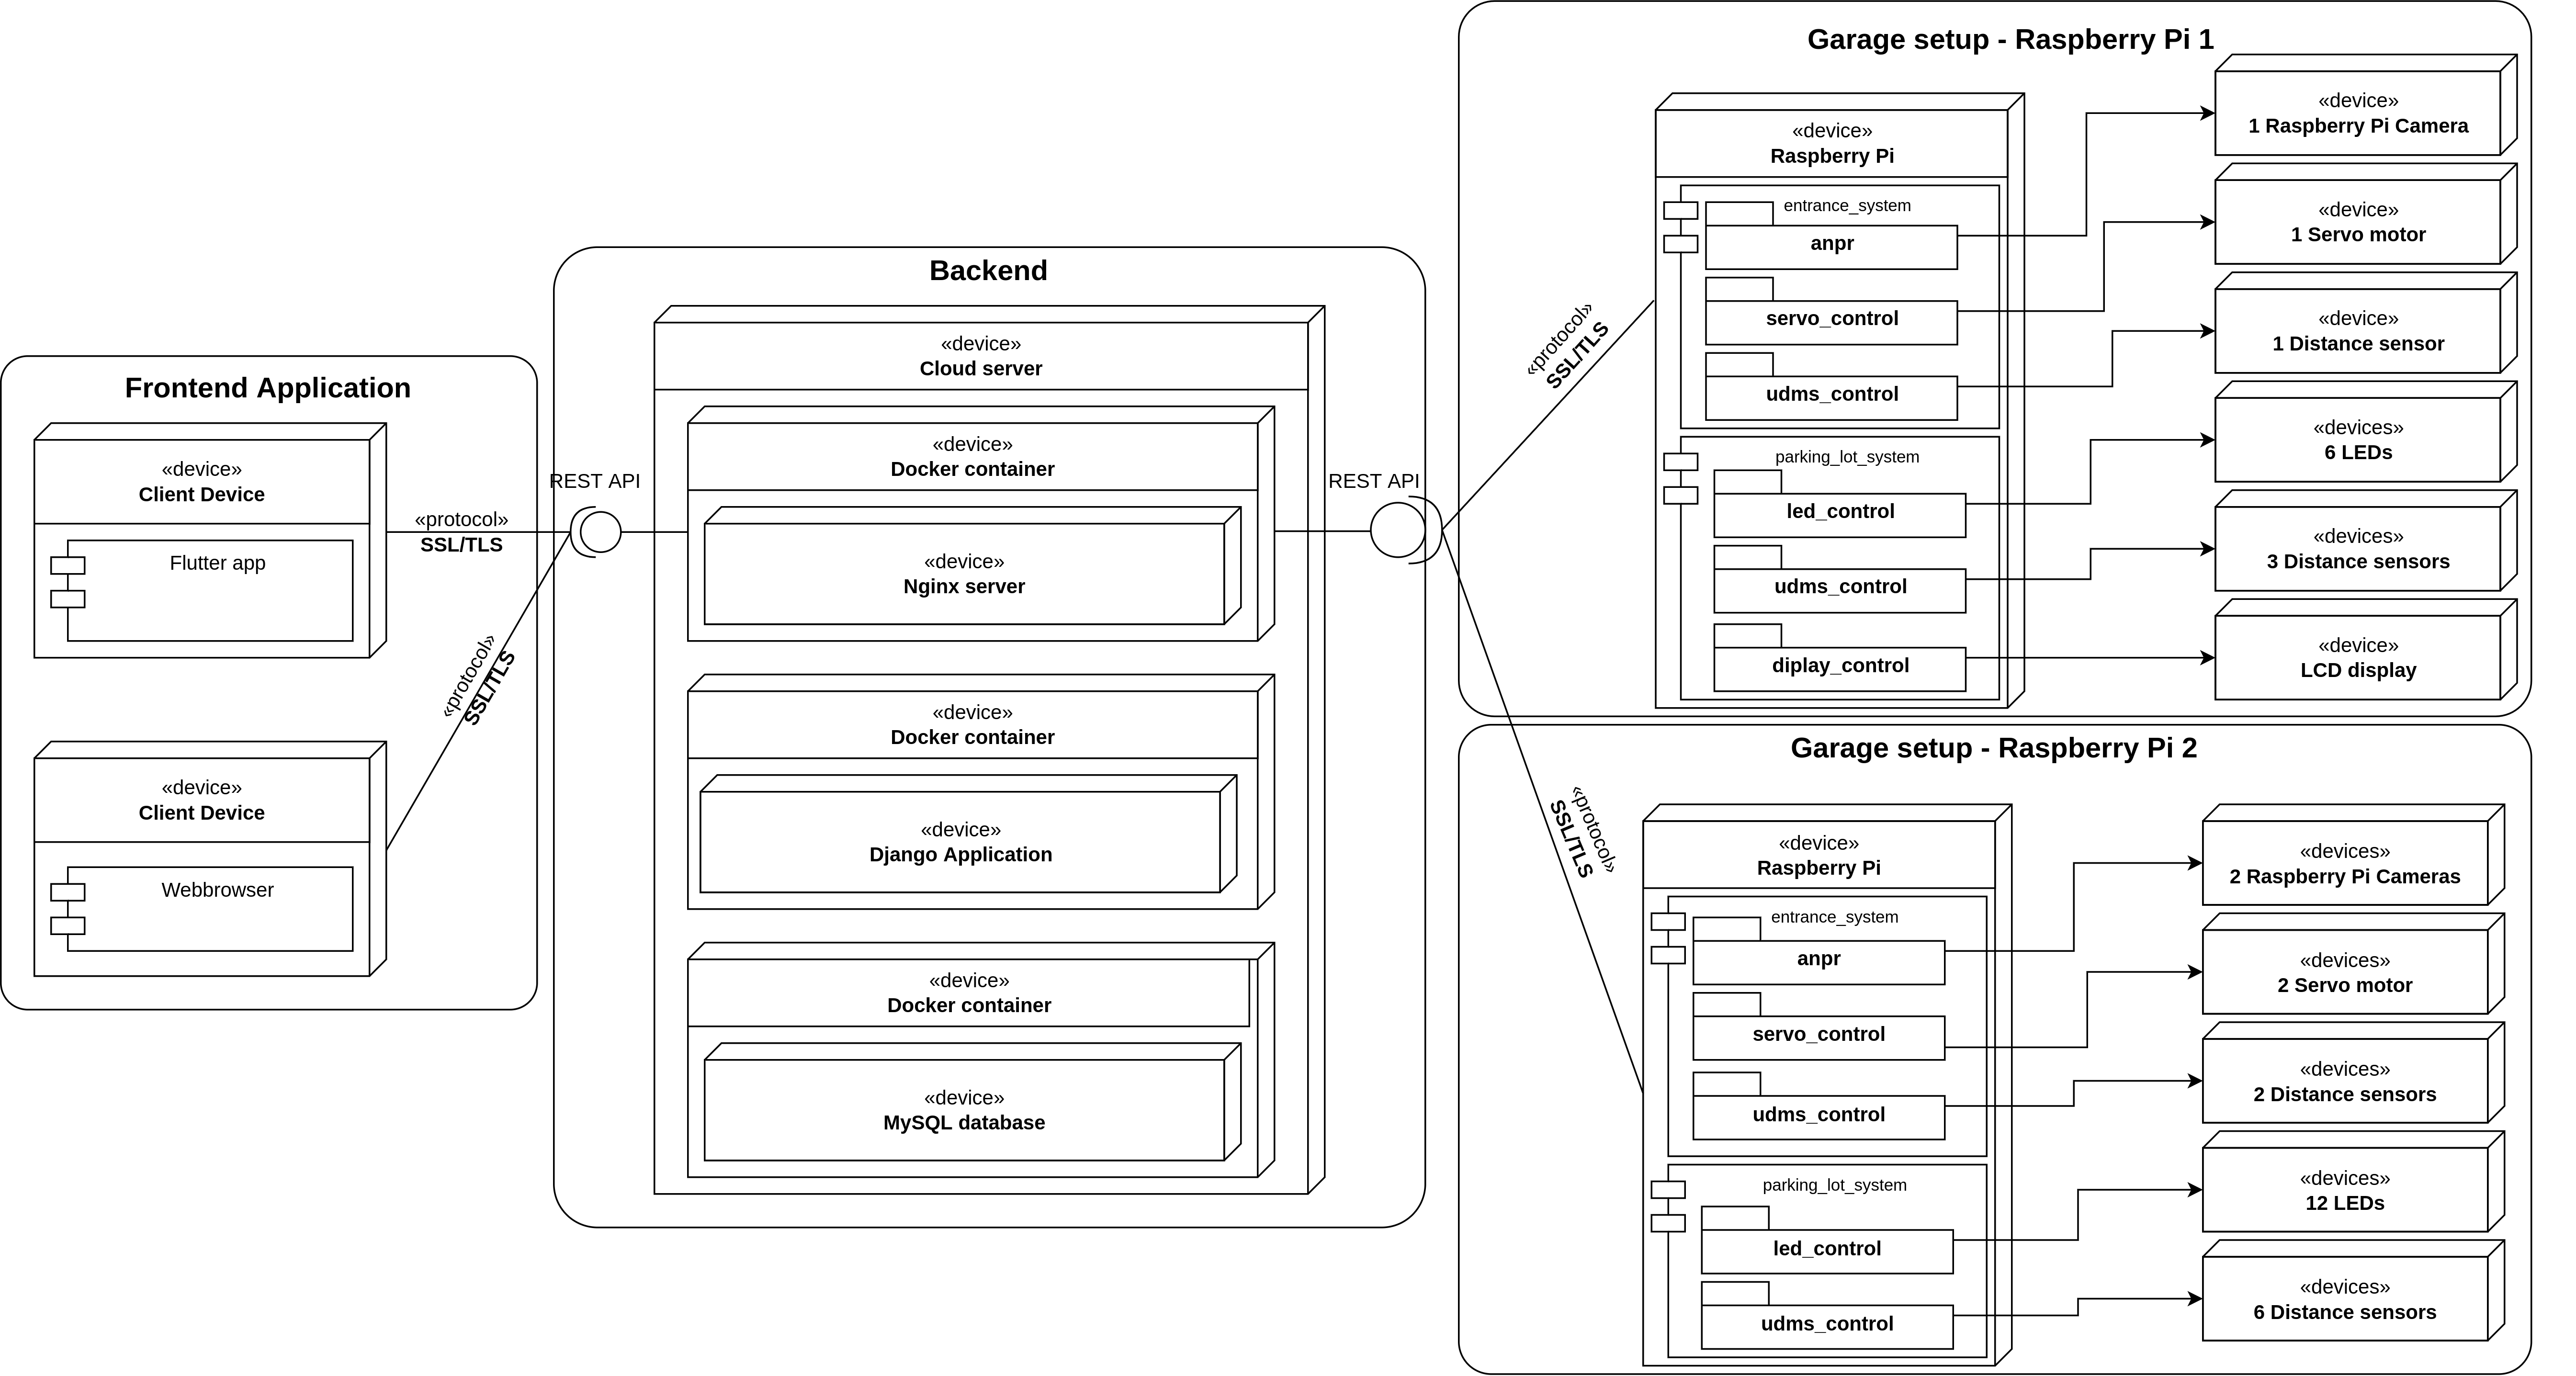
\includegraphics[width=25cm]{images/deployment_diagram.drawio.png}
    \caption{General deployment diagram.}
    \label{fig:general-deployment-diagram}
\end{figure}
\end{landscape}

\clearpage
    
\section{App diagrams}\label{app:app-diagram}
\begin{landscape}
   \begin{figure}
    \centering
    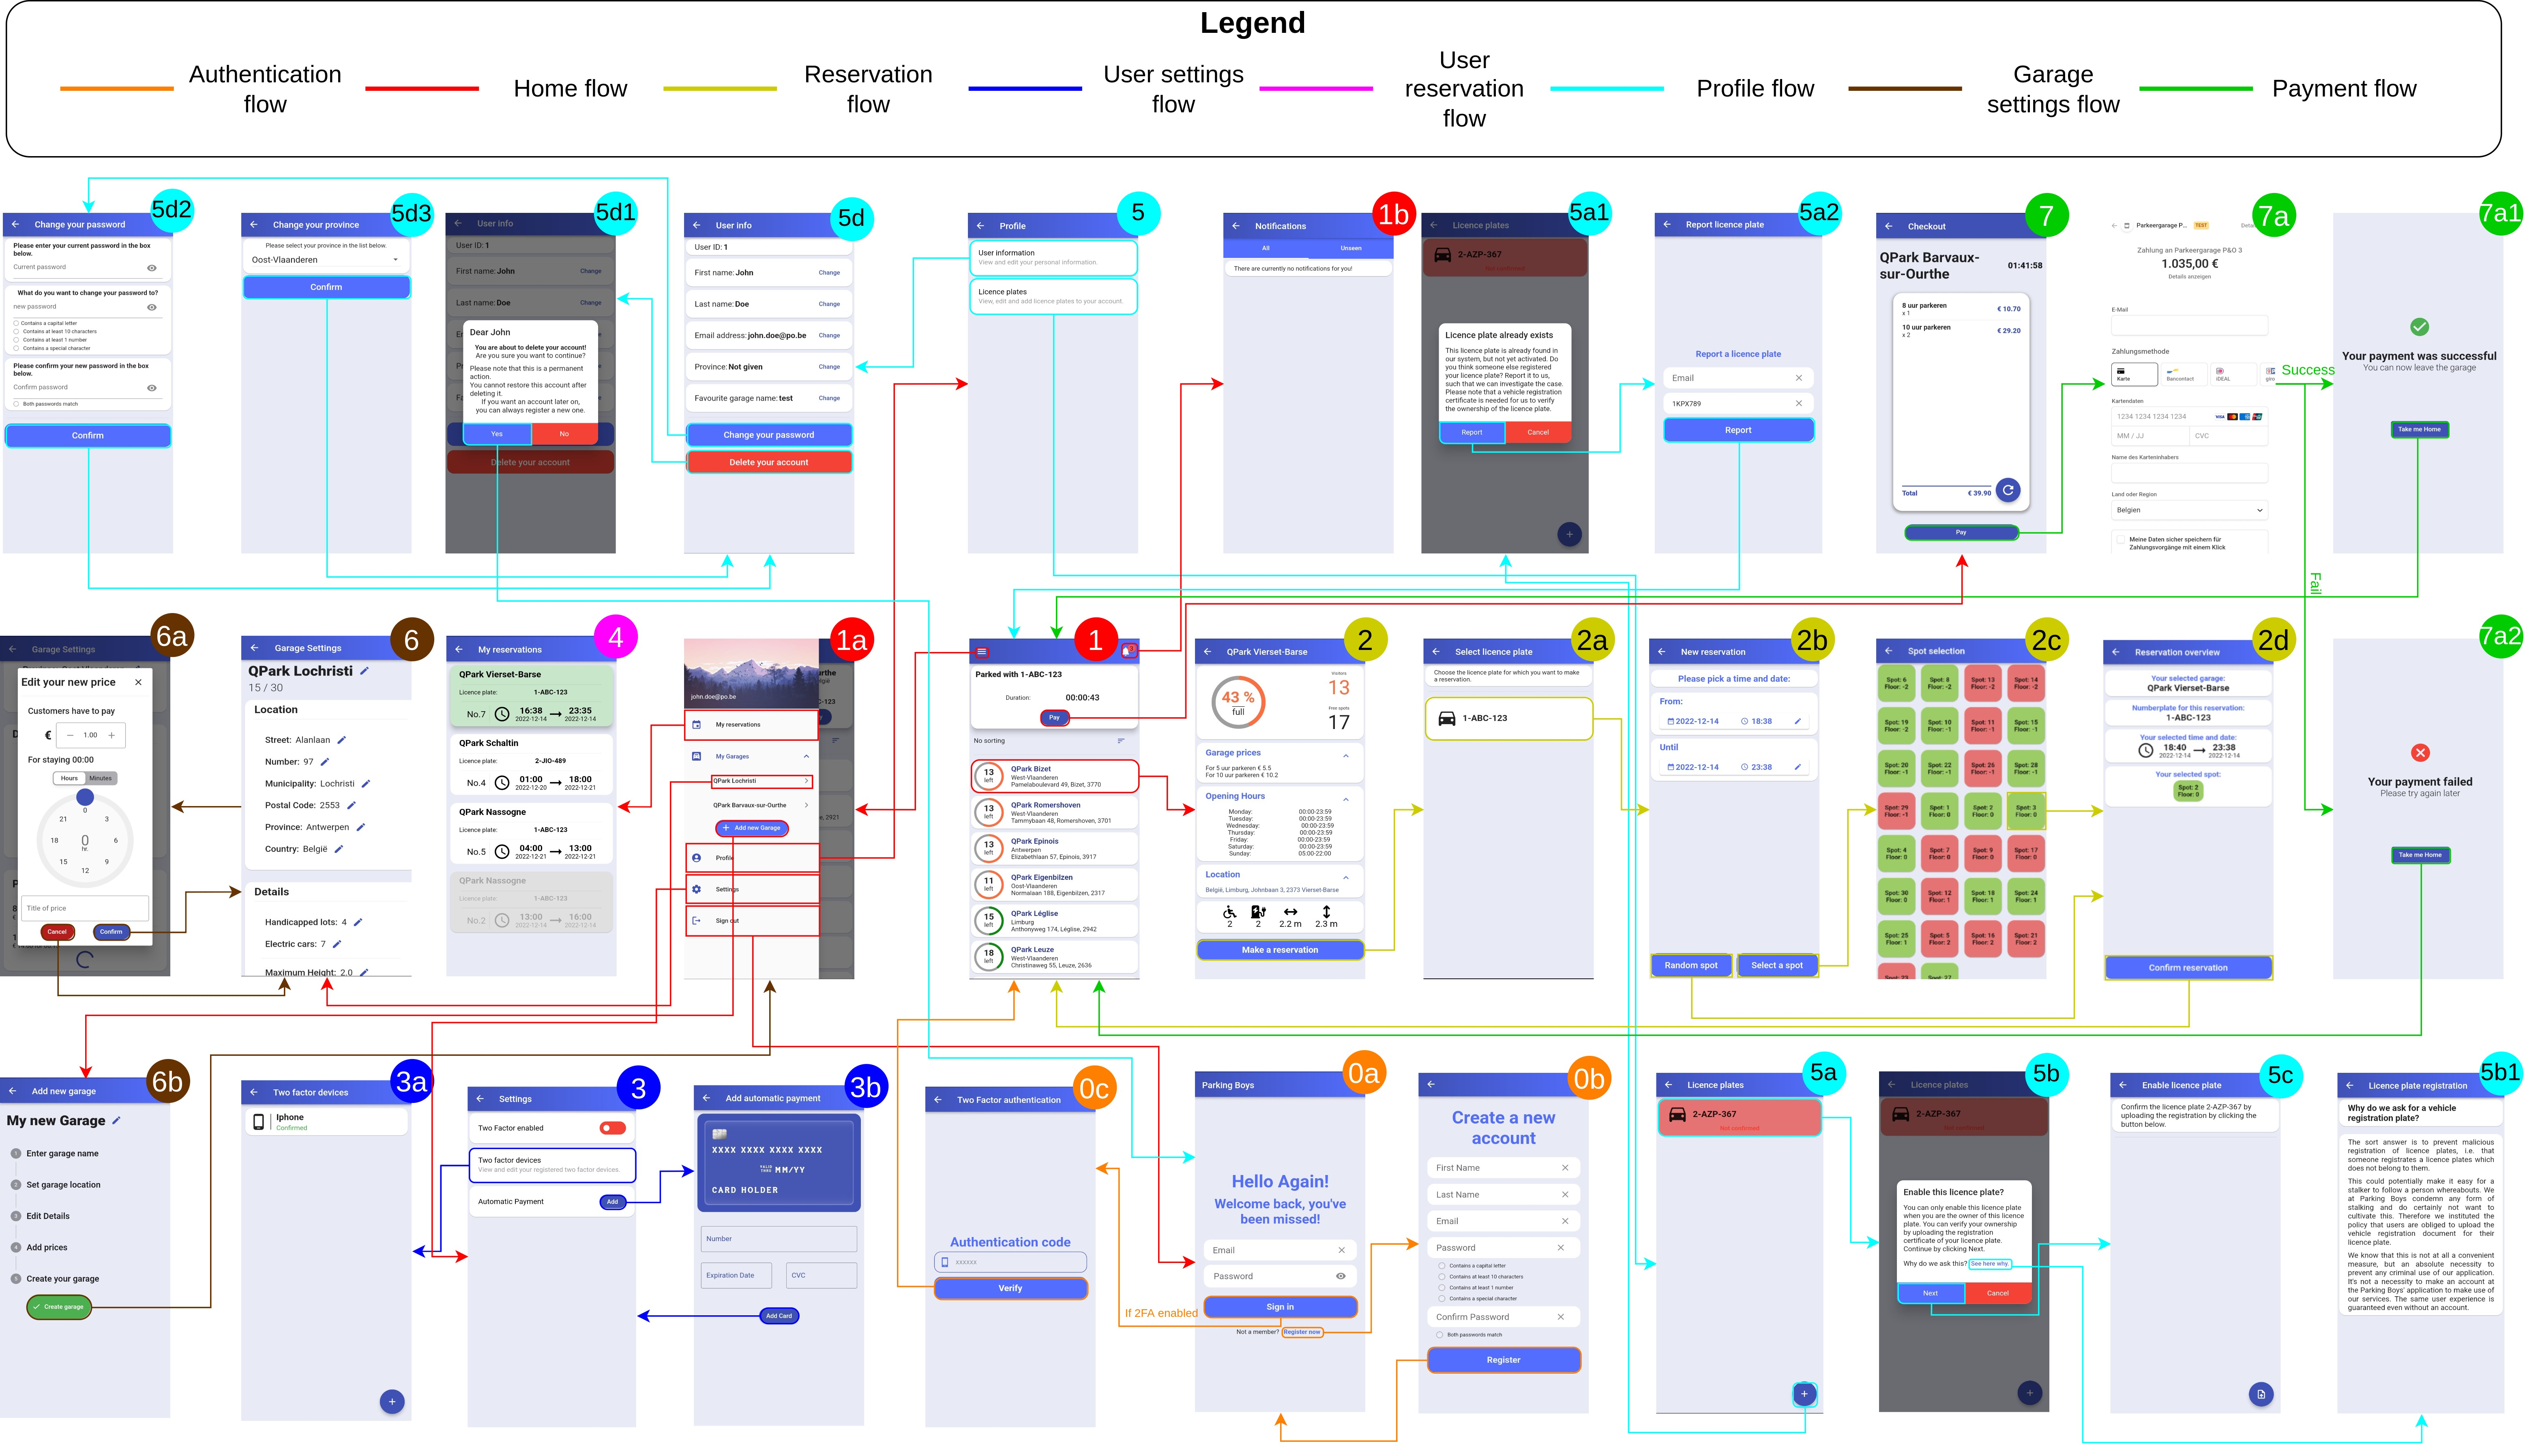
\includegraphics[width=25cm]{images/app_diagram-general.drawio}
    \caption[General app diagram.]{General app diagram which displays the user flow within the frontend application. The pages are enumerated, where a new number indicates a change of flow. Pages with the same number belong to the same logic flow within the application. The routes of the back button are not indicated with an arrow as they represent the reserve direction of the arrow which points to this page.}
    \label{fig:general-app-diagram}
\end{figure}
\end{landscape}

\clearpage
\begin{figure}[hpt]
    \centering
    \includegraphics[width=16cm]{images/app_diagram-auth-flow.drawio.png}
    \caption{App diagram of the authentication flow (Flow 0).}
    \label{fig:auth-flow}
\end{figure}
\begin{figure}[hpt]
    \centering
    \includegraphics[width=16cm]{images/app_diagram-home-flow.drawio.png}
    \caption{App diagram of the home flow (Flow 1).}
    \label{fig:home-flow}
\end{figure}

\clearpage

\begin{figure}[hpt]
    \centering
    \includegraphics[width=14cm]{images/app_diagram-reservation.drawio.png}
    \caption{App diagram of the reservation flow (Flow 2).}
    \label{fig:reservation-flow}
\end{figure}
\begin{figure}[hpt]
    \centering
    \includegraphics[width=14cm]{images/app_diagram-user-settings-flow.drawio.png}
    \caption{App diagram of the user settings flow (Flow 3).}
    \label{fig:user-settings-flow}
\end{figure}
\begin{figure}[!hpt]
    \centering
    \includegraphics[width=14cm]{images/app_diagram-user-reservation-flow.drawio.png}
    \caption{App diagram of the user reservation flow (Flow 4).}
    \label{fig:user-reservation-flow}
\end{figure}

\clearpage

\begin{figure}[hpt]
    \centering
    \includegraphics[width=16cm]{images/app_diagram-profile-flow.drawio.png}
    \caption{App diagram of the profile flow (Flow 5).}
    \label{fig:profile-flow}
\end{figure}
\begin{figure}[hpt]
   \centering
   \includegraphics[width=16cm]{images/app_diagram-garage-settings-flow.drawio.png}
    \caption{App diagram of the garage settings flow (Flow 6).}
   \label{fig:garage-settings-flow}
\end{figure}
\begin{figure}[!hpt]
    \centering
    \includegraphics[width=16cm]{images/app_diagram-payment.drawio.png}
    \caption{App diagram of the payment flow (Flow 7).}
    \label{fig:payment-flow}
\end{figure}

\clearpage

\begin{figure}[htp]
     \centering
     \begin{subfigure}[b]{0.30\textwidth}
         \centering
         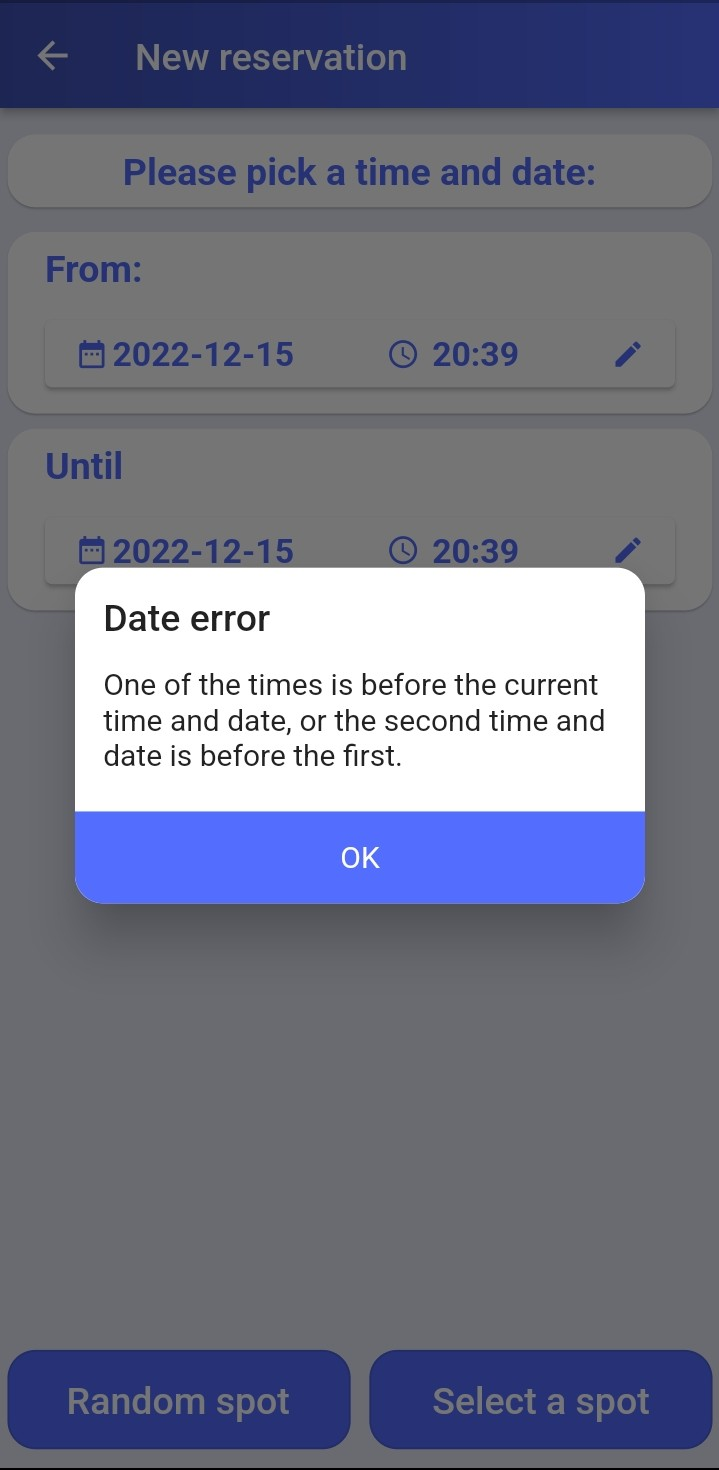
\includegraphics[width=\textwidth]{images/dialog1.jpg}
     \end{subfigure}
     \hfill
     \begin{subfigure}[b]{0.30\textwidth}
         \centering
         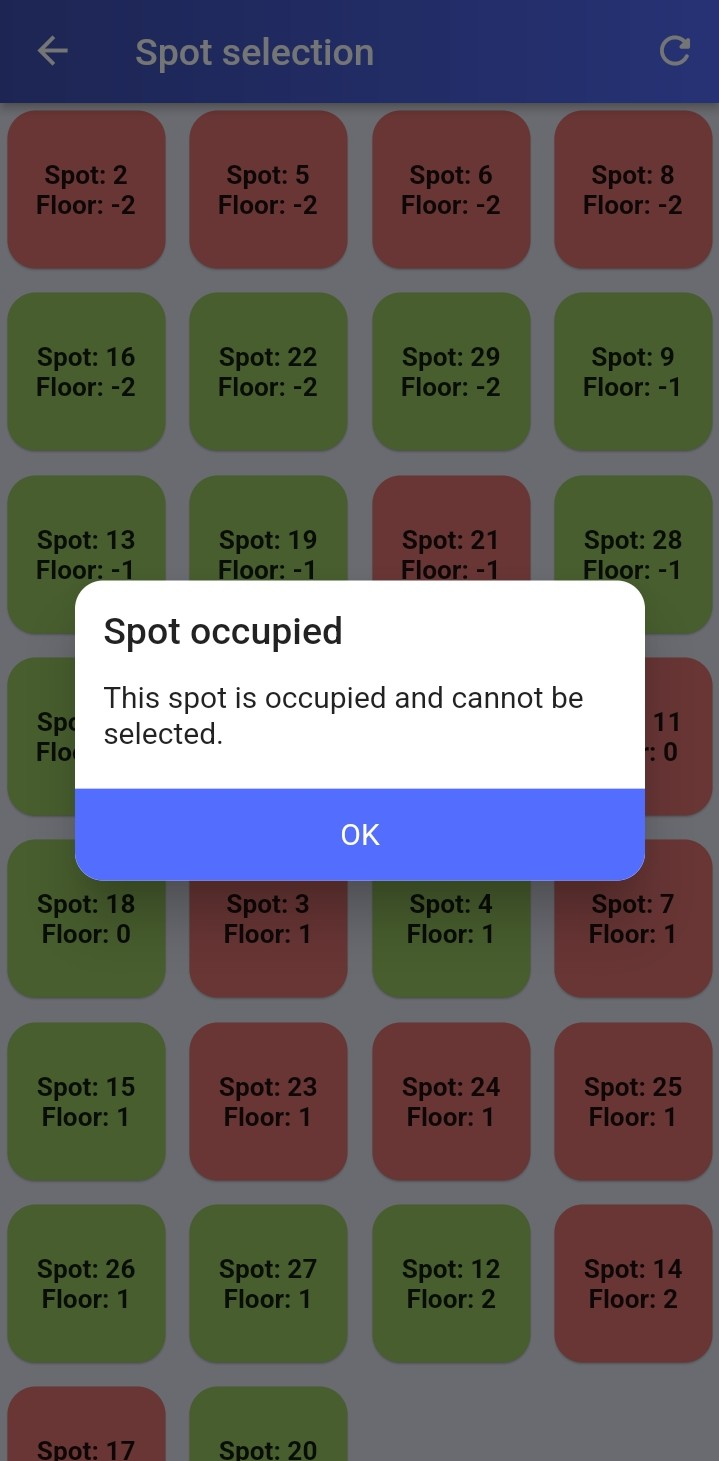
\includegraphics[width=\textwidth]{images/dialog2.jpg}
     \end{subfigure}
        \caption{Examples of error pop ups in the frontend application.}
        \label{fig:error-dialogs}
\end{figure}
\begin{figure}[!htp]
     \centering
     \begin{subfigure}[b]{0.30\textwidth}
         \centering
         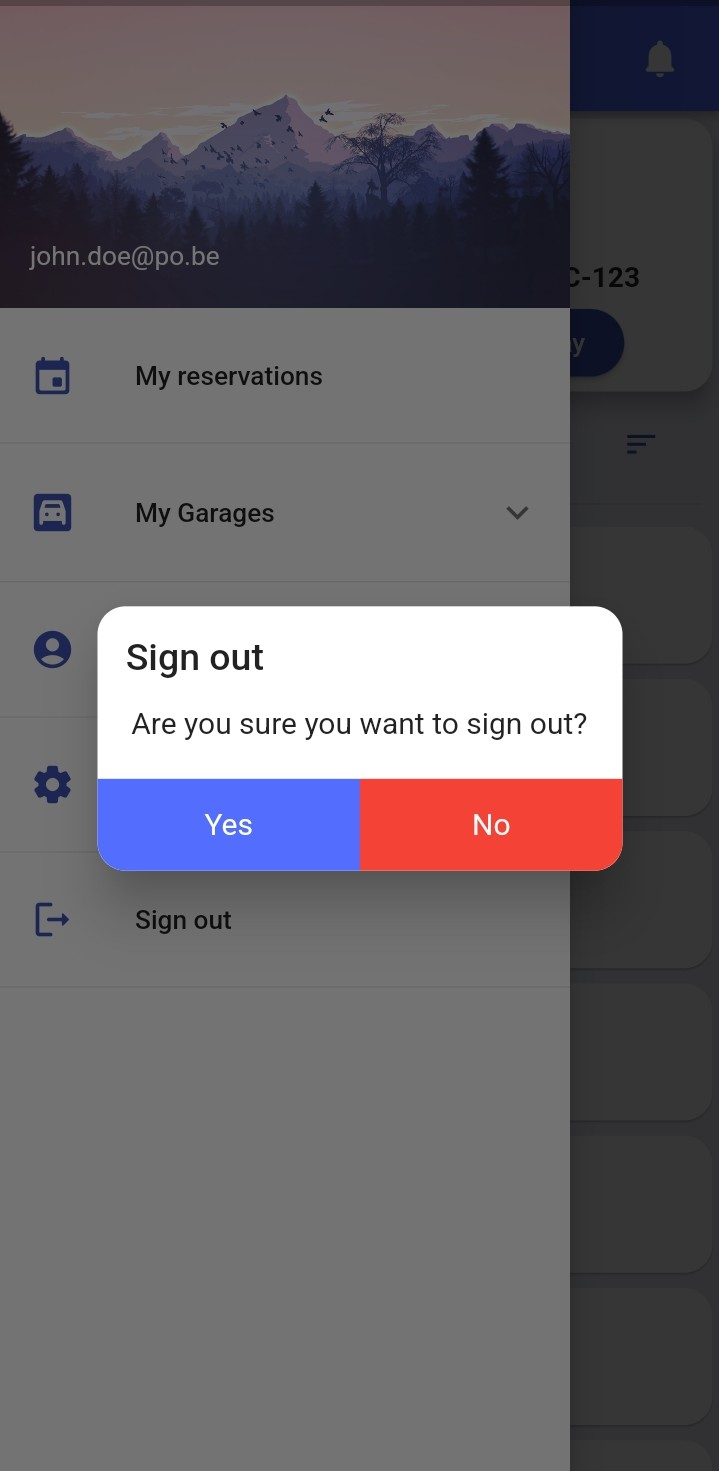
\includegraphics[width=\textwidth]{images/dialog3.jpg}
     \end{subfigure}
     \hfill
     \begin{subfigure}[b]{0.30\textwidth}
         \centering
         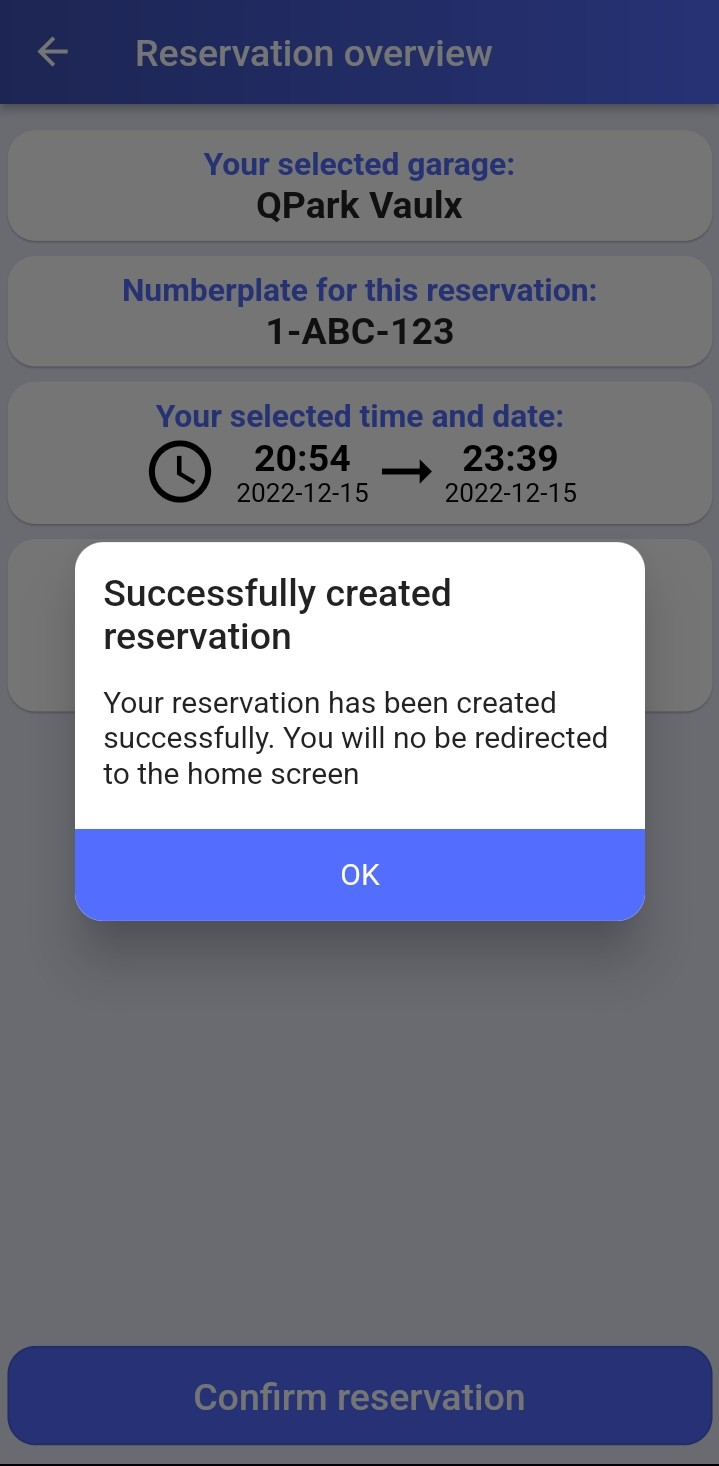
\includegraphics[width=\textwidth]{images/dialog4.jpg}
     \end{subfigure}
        \caption{Examples of information pop ups in the frontend application.}
        \label{fig:information-dialogs}
\end{figure}

\clearpage

\begin{table}[hpt]
    \centering
    \begin{tabular}{|c|c|p{9cm}|}
    \hline
         \textbf{Page code}& \textbf{Page name} & \textbf{Short description} \\
         \hline
         \hline
         0a & Login page & Lets the user enter their email and password and authenticates it with the backend.\\
         \hline 
         0b & Register page & Allows the creation of new accounts by inputting all necessary information by the user.\\
         \hline 
         0c & \ac{2fa} Page & Allows the user to enter the \ac{2fa}-code from their \ac{totp}-device. \\
         \hline 
         \hline
         1 & Home page & Central page in the application which is the entry point for all major flows.\\
         \hline 
         1a & Home banner & Banner which allows the user to navigate to all important flows and to sign out. \\
         \hline 
         \hline
         2 & Garage info page & Provides an overview of all information about a garage, including its occupancy, prices and opening hours. Is the entry point for the reservation flow.\\
         \hline 
         2a & Licence plate selection page & Allows the user to select for which licence plate they want to make a reservation. \\
         \hline 
         2b & Make reservation page & Allows the user to enter their start and end time of the reservation they want to make. Validates them before continuing. \\
         \hline 
         2c & Spot selection page & Allows the user to choose a parking lot for which they want to make a reservation. \\
         \hline 
         2d & Reservation overview page &  Provides an overview of the reservation the user is about to make. On confirm, the user is redirected to the home page \\
         \hline 
         \hline
         3 & Settings page & Entry point for the users altering the user settings. \\
         \hline 
         3a & Two factor devices page & Allows the user to add, update or delete \ac{totp}-devices. \\
         \hline 
         3b & Add automatic payment page& Allows the user to enter their credit card details, which enables automatic payment.\\
         \hline 
         \hline
         4 & User reservation page & Overview of the user's reservations, highlighting the current reservation and disabling past reservations.\\
         \hline 
         \hline
         5 & Profile page & Entry point for altering and viewing user information. \\
         \hline 
         5a & Licence plates page & Allows the user to view, add and confirm licence plates. \\
         \hline 
         5b & Confirm licence plate dialog& Allows the user to choose to enable their licence plate. \\
         \hline 
         5b1 & Registration explication page & Explains the user why a vehicle registration document is necessary for the application to enable their licence plate.\\
         \hline 
         5c & Confirm licence plate page & Allows the user to upload a vehicle registration document to enable their licence plate.\\
         \hline 
         5d & User info page & Allows the user to view and edit their personal information. \\
         \hline 
         5d1 & User deletion pop up & Allows the user to choose if they want to delete their account. \\
         \hline 
         5d2 & Change password page & Allows the user to change their password by entering a new one. \\
         \hline 
         5d3 & Change province page & Allows the user to change their location.\\
         \hline 
         \hline
         6 & Garage settings page & Allows a garage owner to alter the information about their garage, including the parking lots, prices, opening hours and location. \\
         \hline 
         6a & Add prices page & Allows a garage owner to add new prices to their garage. The prices will be synchronised with the Stripe servers.\\
         \hline 
         \hline
         7 & Checkout page & Provides an overview of the due amount and the parked time to the user.\\
         \hline 
         7a & Payment page & Allows the user to pay their parking bill \\
         \hline 
         7a1 & Payment success page & Provides confirmation to the user that their payment was successful. \\
         \hline 
         7a2 & Payment failed page page & Provides confirmation to the user that their payment as unsuccessful. \\
         \hline 
    \end{tabular}
    \caption[An overview of all the different pages in the frontend application.]{An overview of all the different pages in the frontend application, together with their page code and a short description.}
    \label{tab:app-pages}
\end{table}

\clearpage

\section{Mechanical part list}\label{app:part-list}

\begin{table}[htp]
    \centering
    \caption{Overview of all used mechanical components and their model number.}
    \begin{tabular}{|c|c|c|}
        \hline
         \textbf{Component name} & \textbf{Model number} & \textbf{Amount}  \\
         \hline
         \hline
         Raspberry Pi & Model 3B & 2 \\
         \hline
         \textsc{dorhea} Raspberry Pi Mini Kamera & \textsc{he0304-002} & 2 \\
         \hline
         Ultrasonic distance measuring sensor & \textsc{hc-sr04} & 8 \\
         \hline
         \textsc{Micro servo motor} & \textsc{oky8003} & 2 \\
         \hline
         Red \textsc{led} ($3 \ \text{mm}$) & \textsc{com-00533} & 6 \\
         \hline
         Green \textsc{led} ($3 \ \text{mm}$) & \textsc{com-09560} & 6 \\
         \hline
         Resistors ($20 \ \text{k}\Omega$) & \textsc{sfr2500002002fr500} & 12 \\
         \hline
         Jumper cables & / & $\approx 40$ \\
         \hline
         Raspberry Pi camera extension cable & \textsc{b087dfJ2rp} & 2 \\
         \hline
         LCD screen & ST7735 & 1
         \\
         \hline
         \end{tabular}
    \label{tab:part_list}
\end{table}
\clearpage

\section{Backend API slugs}\label{app:backend-api-slugs}
\begin{table}[htp]
    \centering
    \begin{tabular}{|l|l|p{7cm}|}
        \hline
         \textbf{Slug} & \textbf{Methods} & \textbf{Short Description}  \\
         \hline
         \hline
         \texttt{api/user} &  \texttt{GET}, \texttt{PUT}, \texttt{DELETE} & Get, update or delete user information.\\
        \hline
        \texttt{api/user/change-password} &  \texttt{PUT} & Update a user's password, provided the old one.\\
        \hline
        \texttt{api/garages} &  \texttt{GET}, \texttt{POST}& Get all the available garages or post a new one.\\
        \hline
        \texttt{api/garage/<int:pk>} &  \texttt{GET}, \texttt{PUT}, \texttt{DELETE
        } & Get, update or delete information about a single garage.\\
        \hline
        \texttt{api/prices/<int:pk>} &  \texttt{GET}, \texttt{PUT}, \texttt{DELETE
        } & Get all the prices for a garage with id \texttt{pk}.\\
        \hline
        \texttt{api/opening-hours/<int:pk>} &  \texttt{GET}, \texttt{POST} & Get all the opening hours for a garage with id \texttt{pk} or add a new one.\\
        \hline
        \texttt{api/opening-hour/<int:pk>} &  \texttt{PUT}, \texttt{DELETE} & Update or delete opening hours with id \texttt{pk}.\\
        \hline
        \texttt{api/parking-lots/<int:pk>} &  \texttt{GET} & Get all the parking lots for a garage with id \texttt{pk}.\\
        \hline
        \texttt{api/parking-lot/<int:pk>} &  \texttt{GET}, \texttt{PUT}, \texttt{DELETE
        } & Get update or delete a parking lot with id \texttt{pk}. \\
        \hline
        \texttt{api/assign-parking-lot/<int:pk>} &  \texttt{GET} & Get a random free parking lot in the garage with id \texttt{pk}, given a start and end date. \\
        \hline
        \texttt{api/garage-settings/<int:pk>} &  \texttt{GET}, \texttt{PUT}, \texttt{DELETE
        } & Get, update or delete the garage settings of a garage with id \texttt{pk}.\\
        \hline
        \texttt{api/licence-plates} &  \texttt{GET}, \texttt{POST} & Get all licence plates for a user or add a new one.\\
        \hline
        \texttt{api/licence-plate/<int:pk>} &  \texttt{GET}, \texttt{PUT}, \texttt{DELETE} & Get, update or delete a licence plate with id \texttt{pk}. \\
        \hline
        \texttt{api/reservations} &  \texttt{GET}, \texttt{POST} & Get all user's reservations or add a new one.\\
        \hline
        \texttt{api/reservation/<int:pk>} &  \texttt{PUT}, \texttt{DELETE
        } & Update or delete a notification with id \texttt{pk}.\\
        \hline
        \texttt{api/notifications/<int:pk>} &  \texttt{GET} & Get all user's notifications.\\
        \hline
        \texttt{api/notification/<int:pk>} &  \texttt{PUT}, \texttt{DELETE
        } & Update or delete a notification with id \texttt{pk}.\\
        \hline
        \end{tabular}
    \caption{Overview of all general \ac{url} slugs which are supported by the backend application.}
    \label{tab:my_label}
\end{table}


\begin{table}[htp]
    \centering
    \begin{tabular}{|l|l|p{7cm}|}
    \hline
    \textbf{Slug} & \textbf{Methods} & \textbf{Short Description}  \\
    \hline
    \hline
        \texttt{api/auth/login} &  \texttt{POST} & Login a user given a email and password.\\
        \hline
        \texttt{api/auth/logout} &  \texttt{POST} & Logout a user, deleting its auth token.\\
        \hline
        \texttt{api/auth/activate-account} &  \texttt{GET} & Activate a user's account.\\
        \hline
        \texttt{api/auth/totp/disable} &  \texttt{POST} & Disable \ac{2fa} for a user.\\
        \hline
        \texttt{api/auth/totp} &  \texttt{GET}, \texttt{POST} & Get all the user's \ac{totp}-devices or add a new one.\\
        \hline
        \texttt{api/auth/totp/<int:pk>} &  \texttt{PUT}, \texttt{DELETE} & Update or delete a \ac{totp}-device with id \texttt{pk}.\\
        \hline
        \texttt{api/auth/totp/login/<int:code>} & \texttt{POST} & Post the \ac{2fa}-code to verify the user (\texttt{code} is a six-digit number).\\
        \hline
    \end{tabular}
    \caption{Overview of all \ac{url} slugs for authentication which are supported by the backend application.}
    \label{tab:my_label}
\end{table}


\begin{table}[htp]
    \centering
    \begin{tabular}{|l|l|p{7cm}|}
        \hline
    \textbf{Slug} & \textbf{Methods} & \textbf{Short Description}  \\
    \hline
        \hline
        \texttt{api/rpi/images} &  \texttt{POST} & Post the image taken by the Raspberry Pi to the backend for image analysis.\\
        \hline
        \texttt{api/rpi/parking-lot} &  \texttt{GET} & Get the parking lots from the garage where the Raspberry Pi is installed.\\
        \hline
            \end{tabular}
    \caption{Overview of all \ac{url} slugs for the local garage system, which are supported by the backend application.}
    \label{tab:url-rpi}
\end{table}


\begin{table}[htp]
    \centering
    \begin{tabular}{|l|l|p{7cm}|}
        \hline
    \textbf{Slug} & \textbf{Methods} & \textbf{Short Description}  \\
    \hline
        \hline
        \texttt{api/checkout/create-session} &  \texttt{POST} & Create a checkout session for the user to pay.\\
        \hline
        \texttt{api/checkout/preview} &  \texttt{GET} & Get the items which the user has to pay (i.e. time quantities parked).\\
        \hline
        \texttt{api/checkout/webhook} &  \texttt{POST} & Listen to incoming requests from the Stripe servers for checkout updates.\\
        \hline
        \texttt{api/stripe-connection} &  \texttt{POST} & Add or remove customers from Stripe.\\
        \hline
        \texttt{api/invoice/webhook} &  \texttt{POST} & Post the image taken by the Raspberry Pi to the backend for image analysis.\\
        \hline
        \texttt{api/rpi/parking-lot} &  \texttt{GET} & Listen to invoice updates from the Stripe servers.\\
        \hline
    \end{tabular}
    \caption{Overview of all \ac{url} slugs for payment which are supported by the backend application.}
    \label{tab:url-payment}
\end{table}

\section{Flowcharts}\label{app:flowcharts}

\begin{figure}[htp]
    \centering
    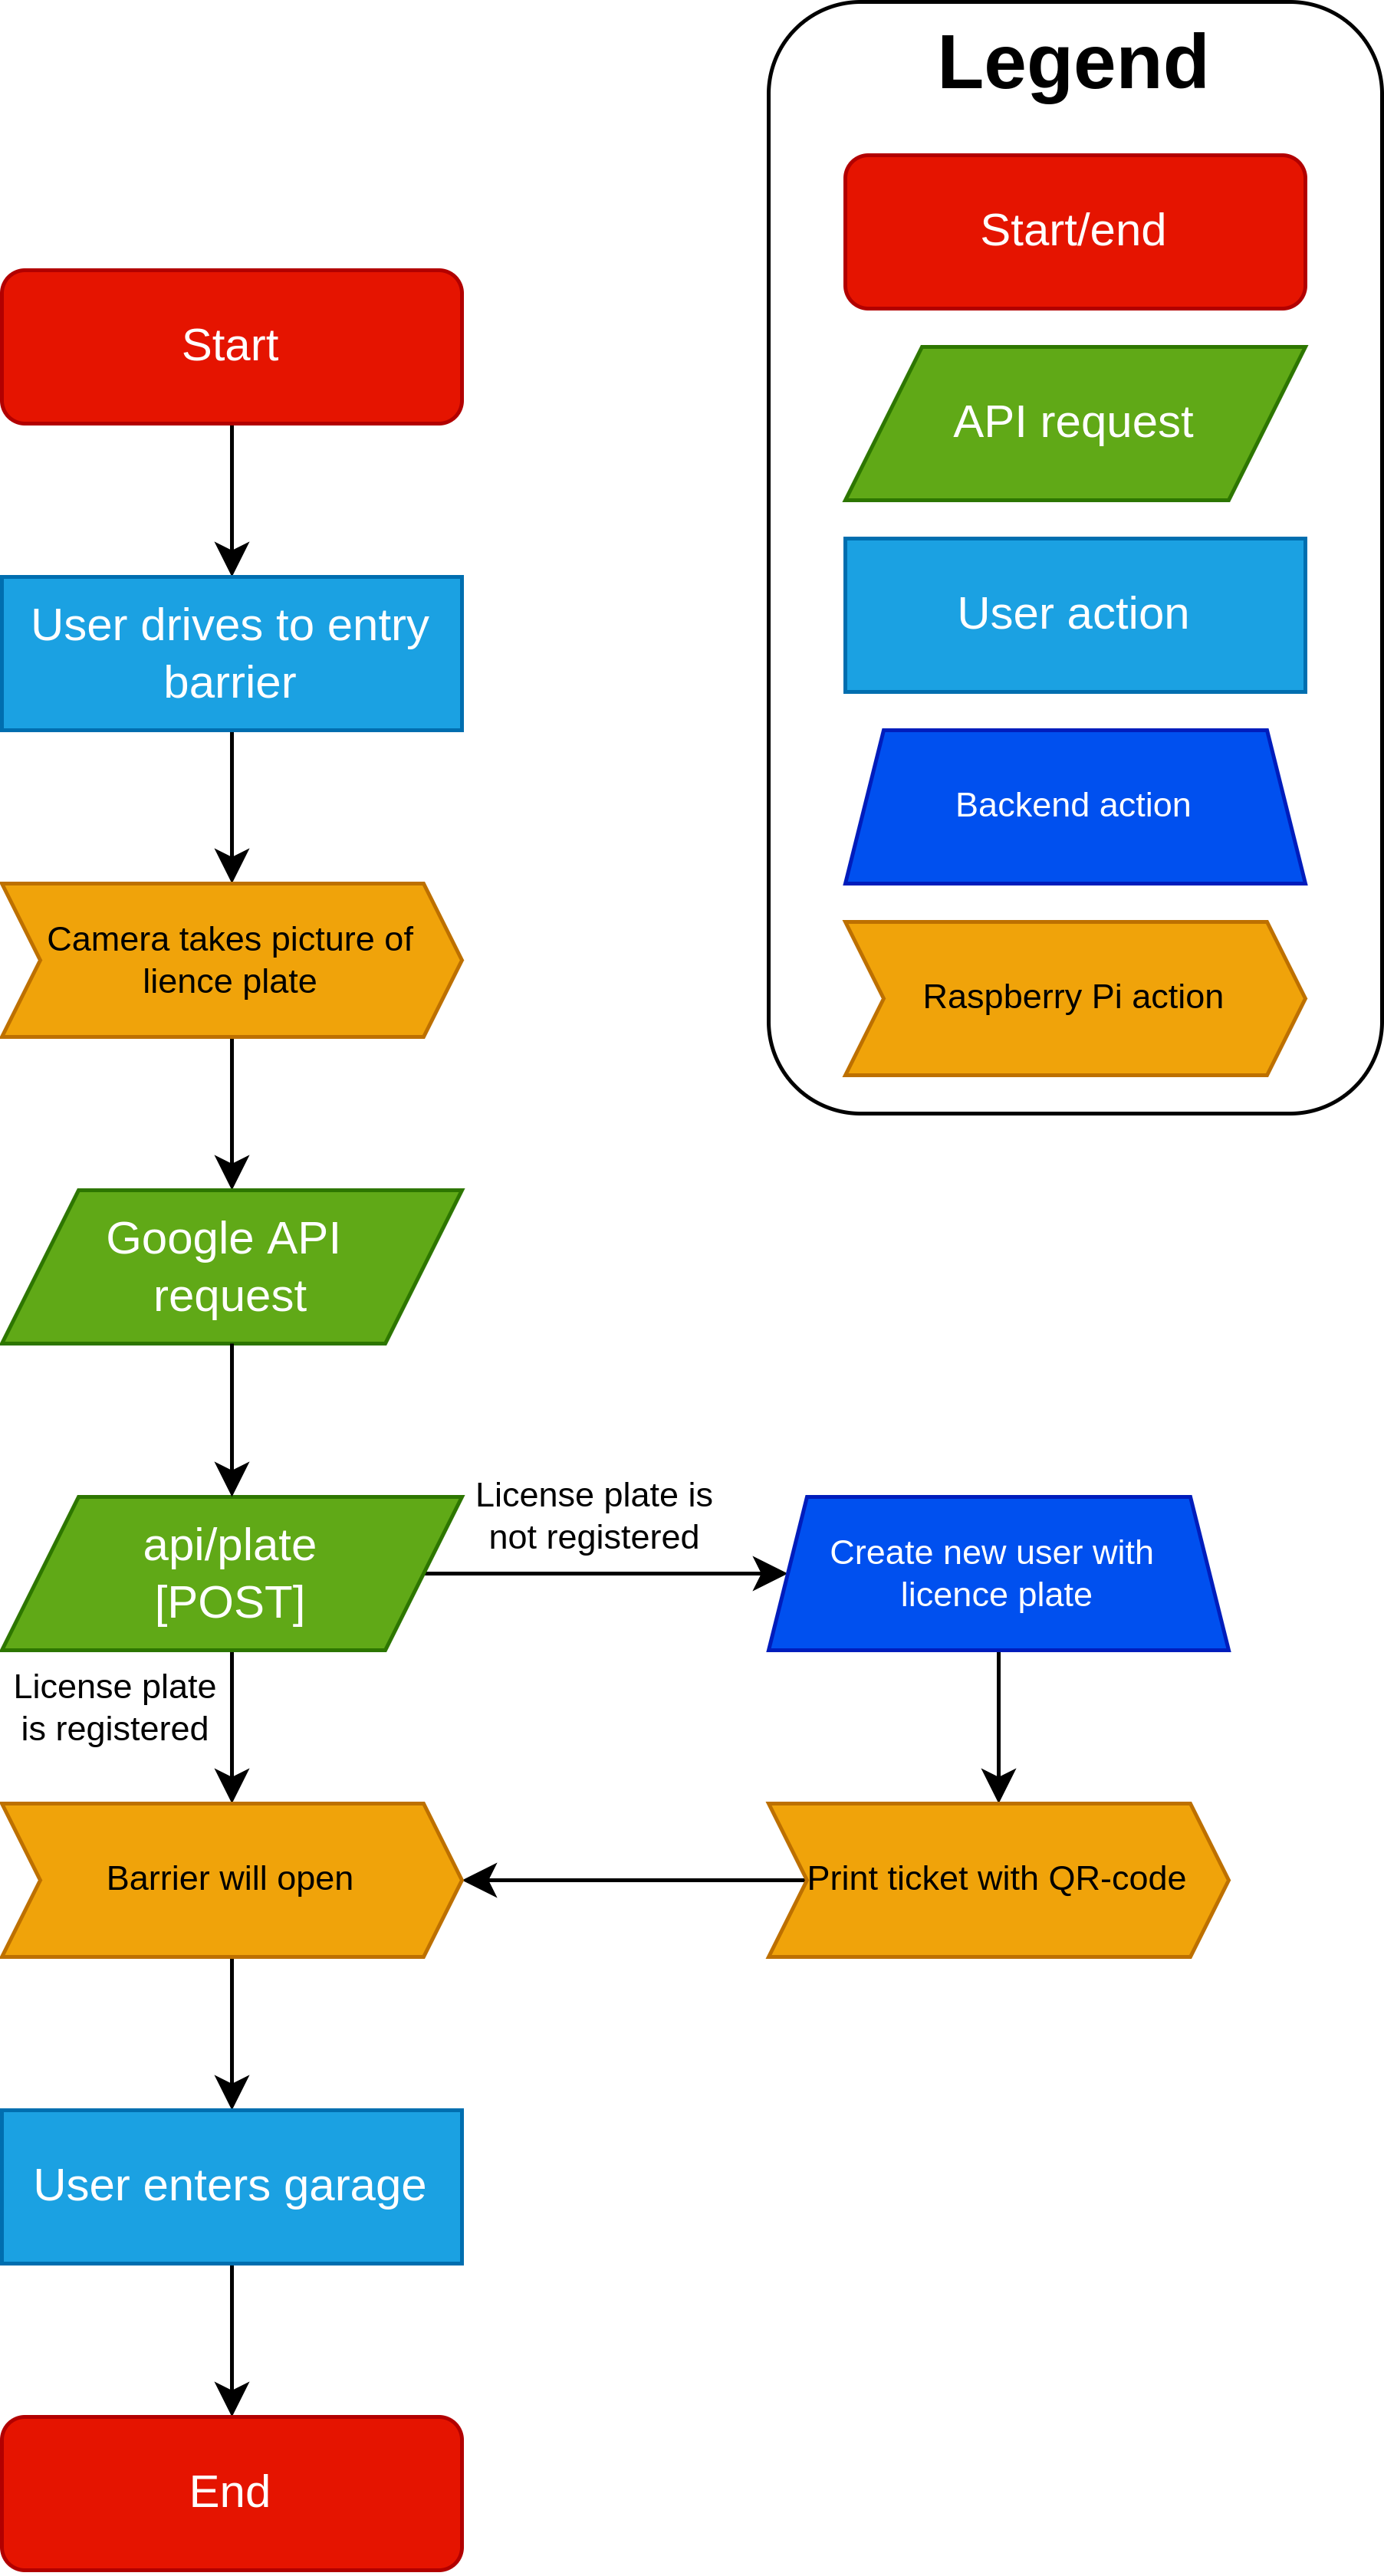
\includegraphics[width=7cm]{images/garage_enter.drawio.png}
    \caption{Flowchart of the entering process of the garage in both hardware, software and user terms.}
    \label{fig:garage-enter}
\end{figure}

\begin{figure}[htp]
    \centering
    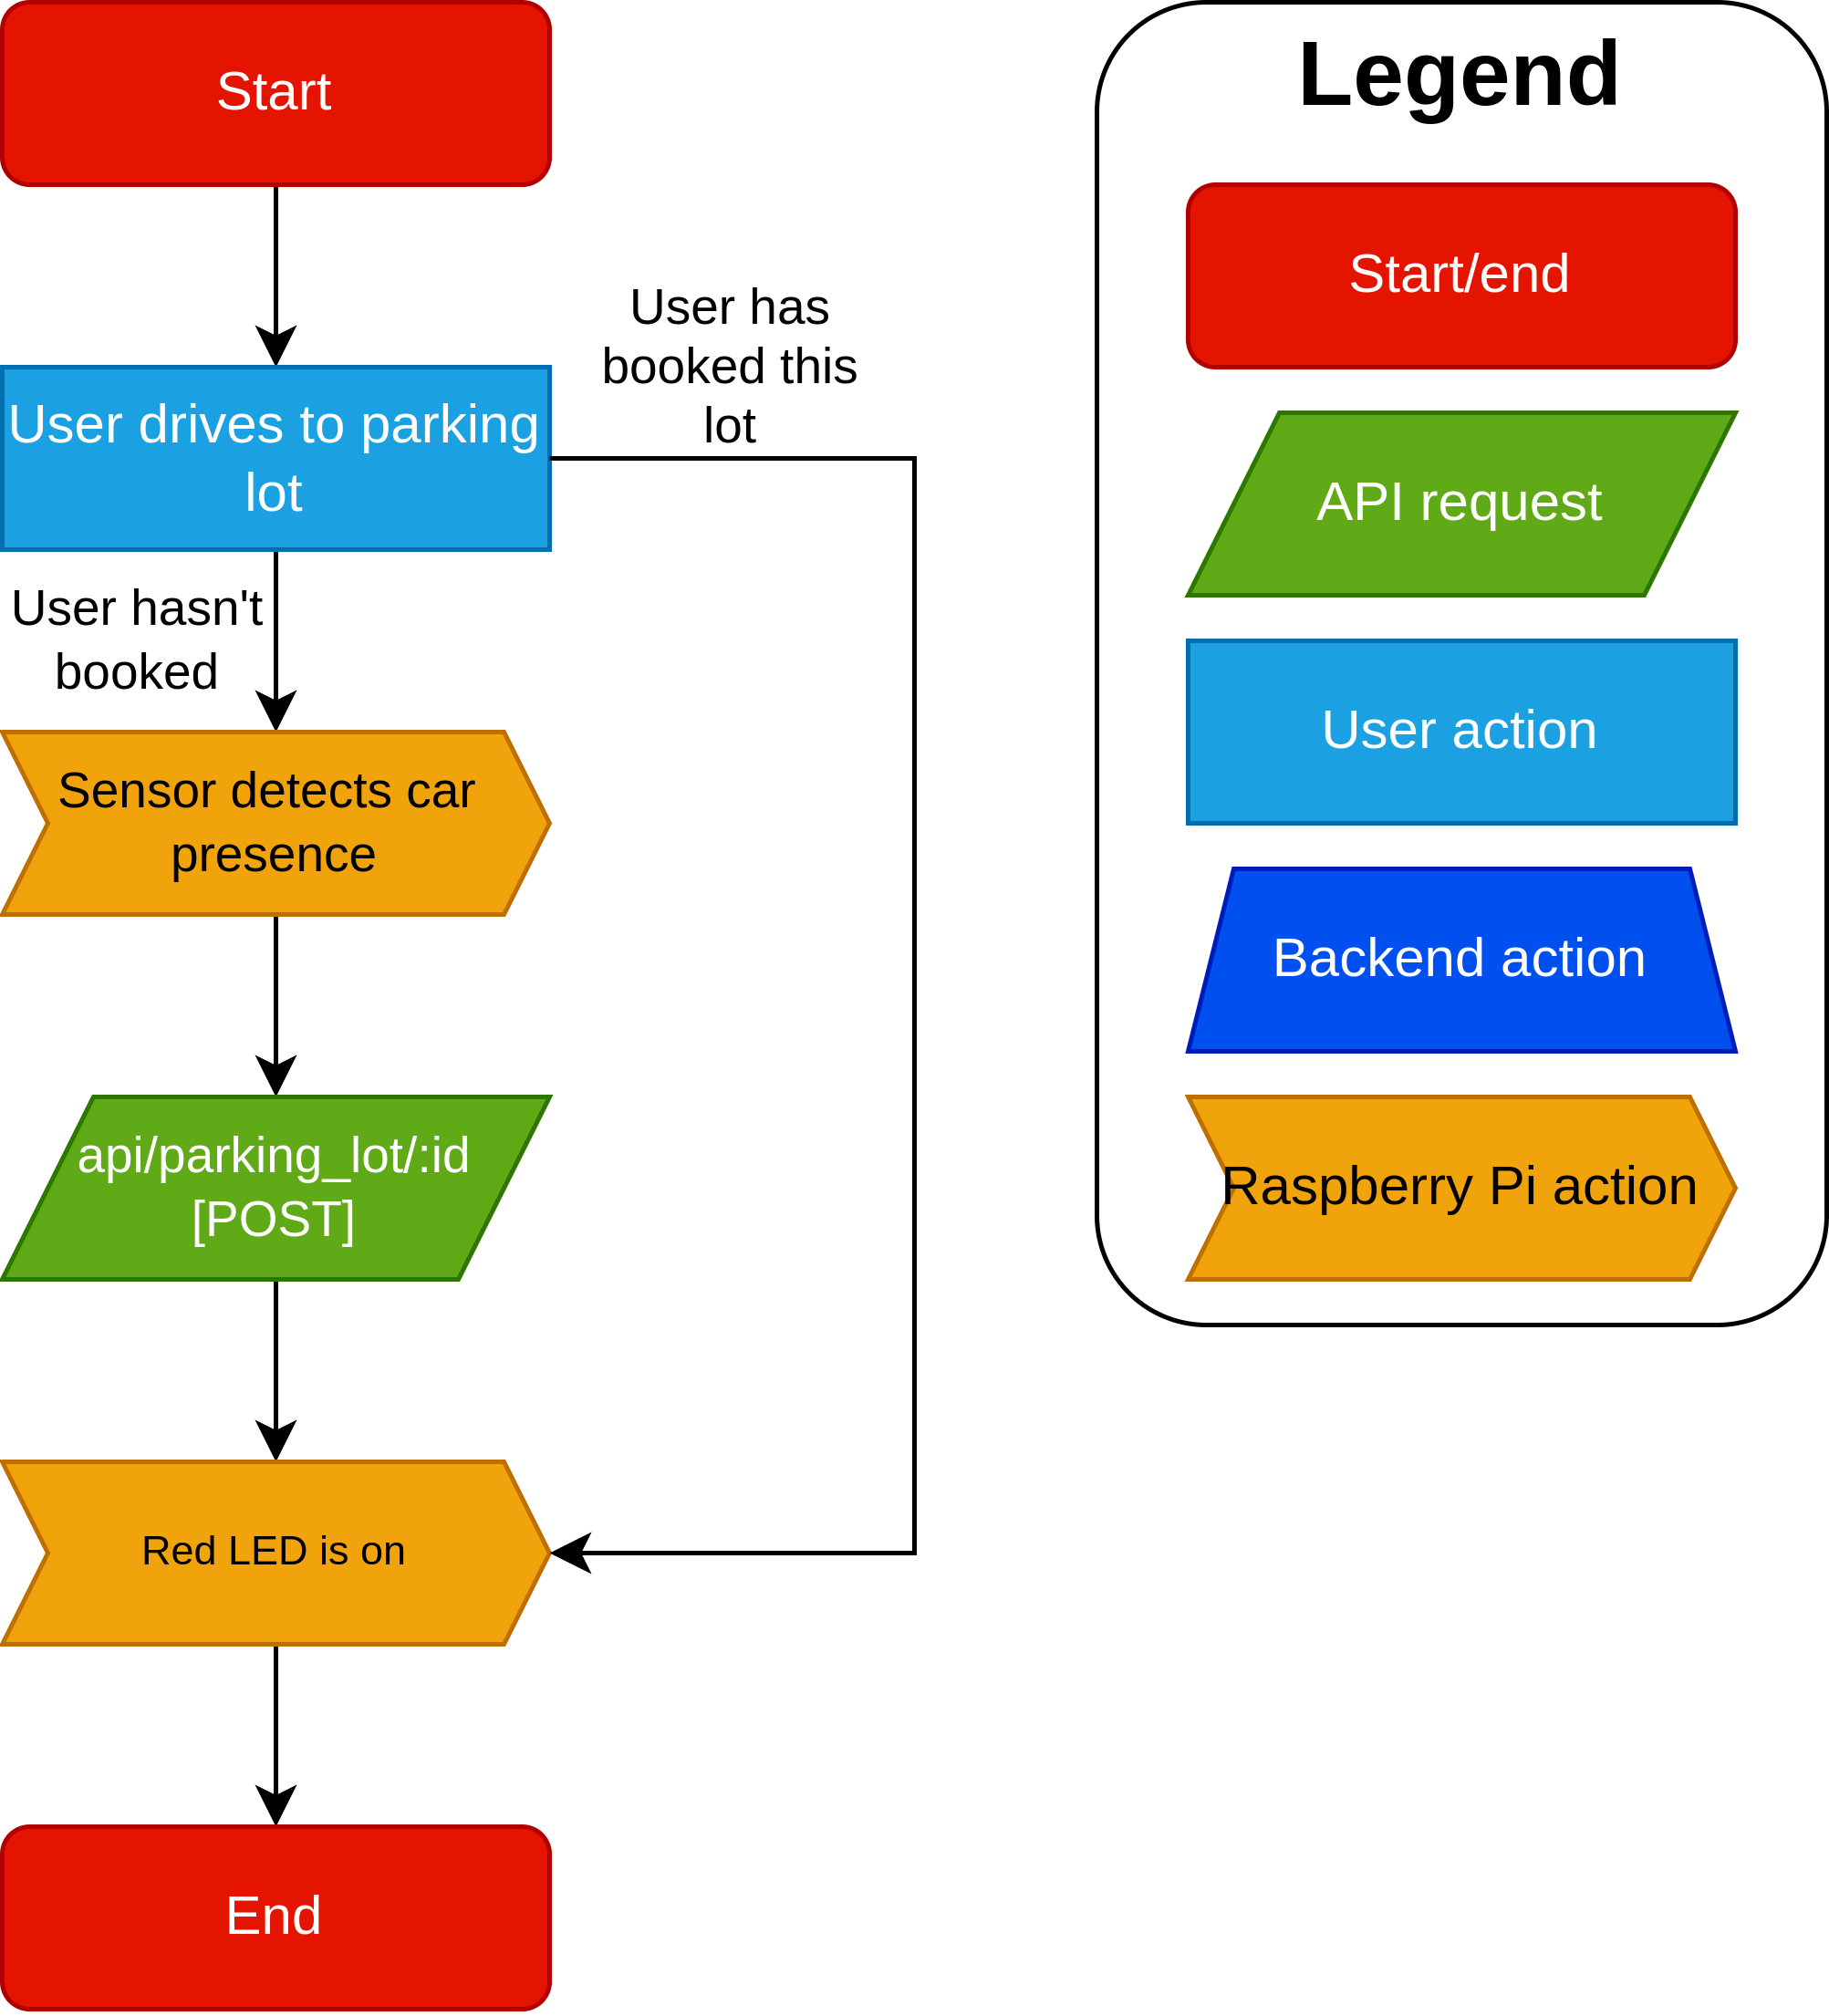
\includegraphics[width=7cm]{images/car_detection.drawio.png}
    \caption{Flowchart of the car detection process of the garage in both hardware, software and user terms.}
    \label{fig:car-detection}
\end{figure}

\begin{figure}[htp]
    \centering
    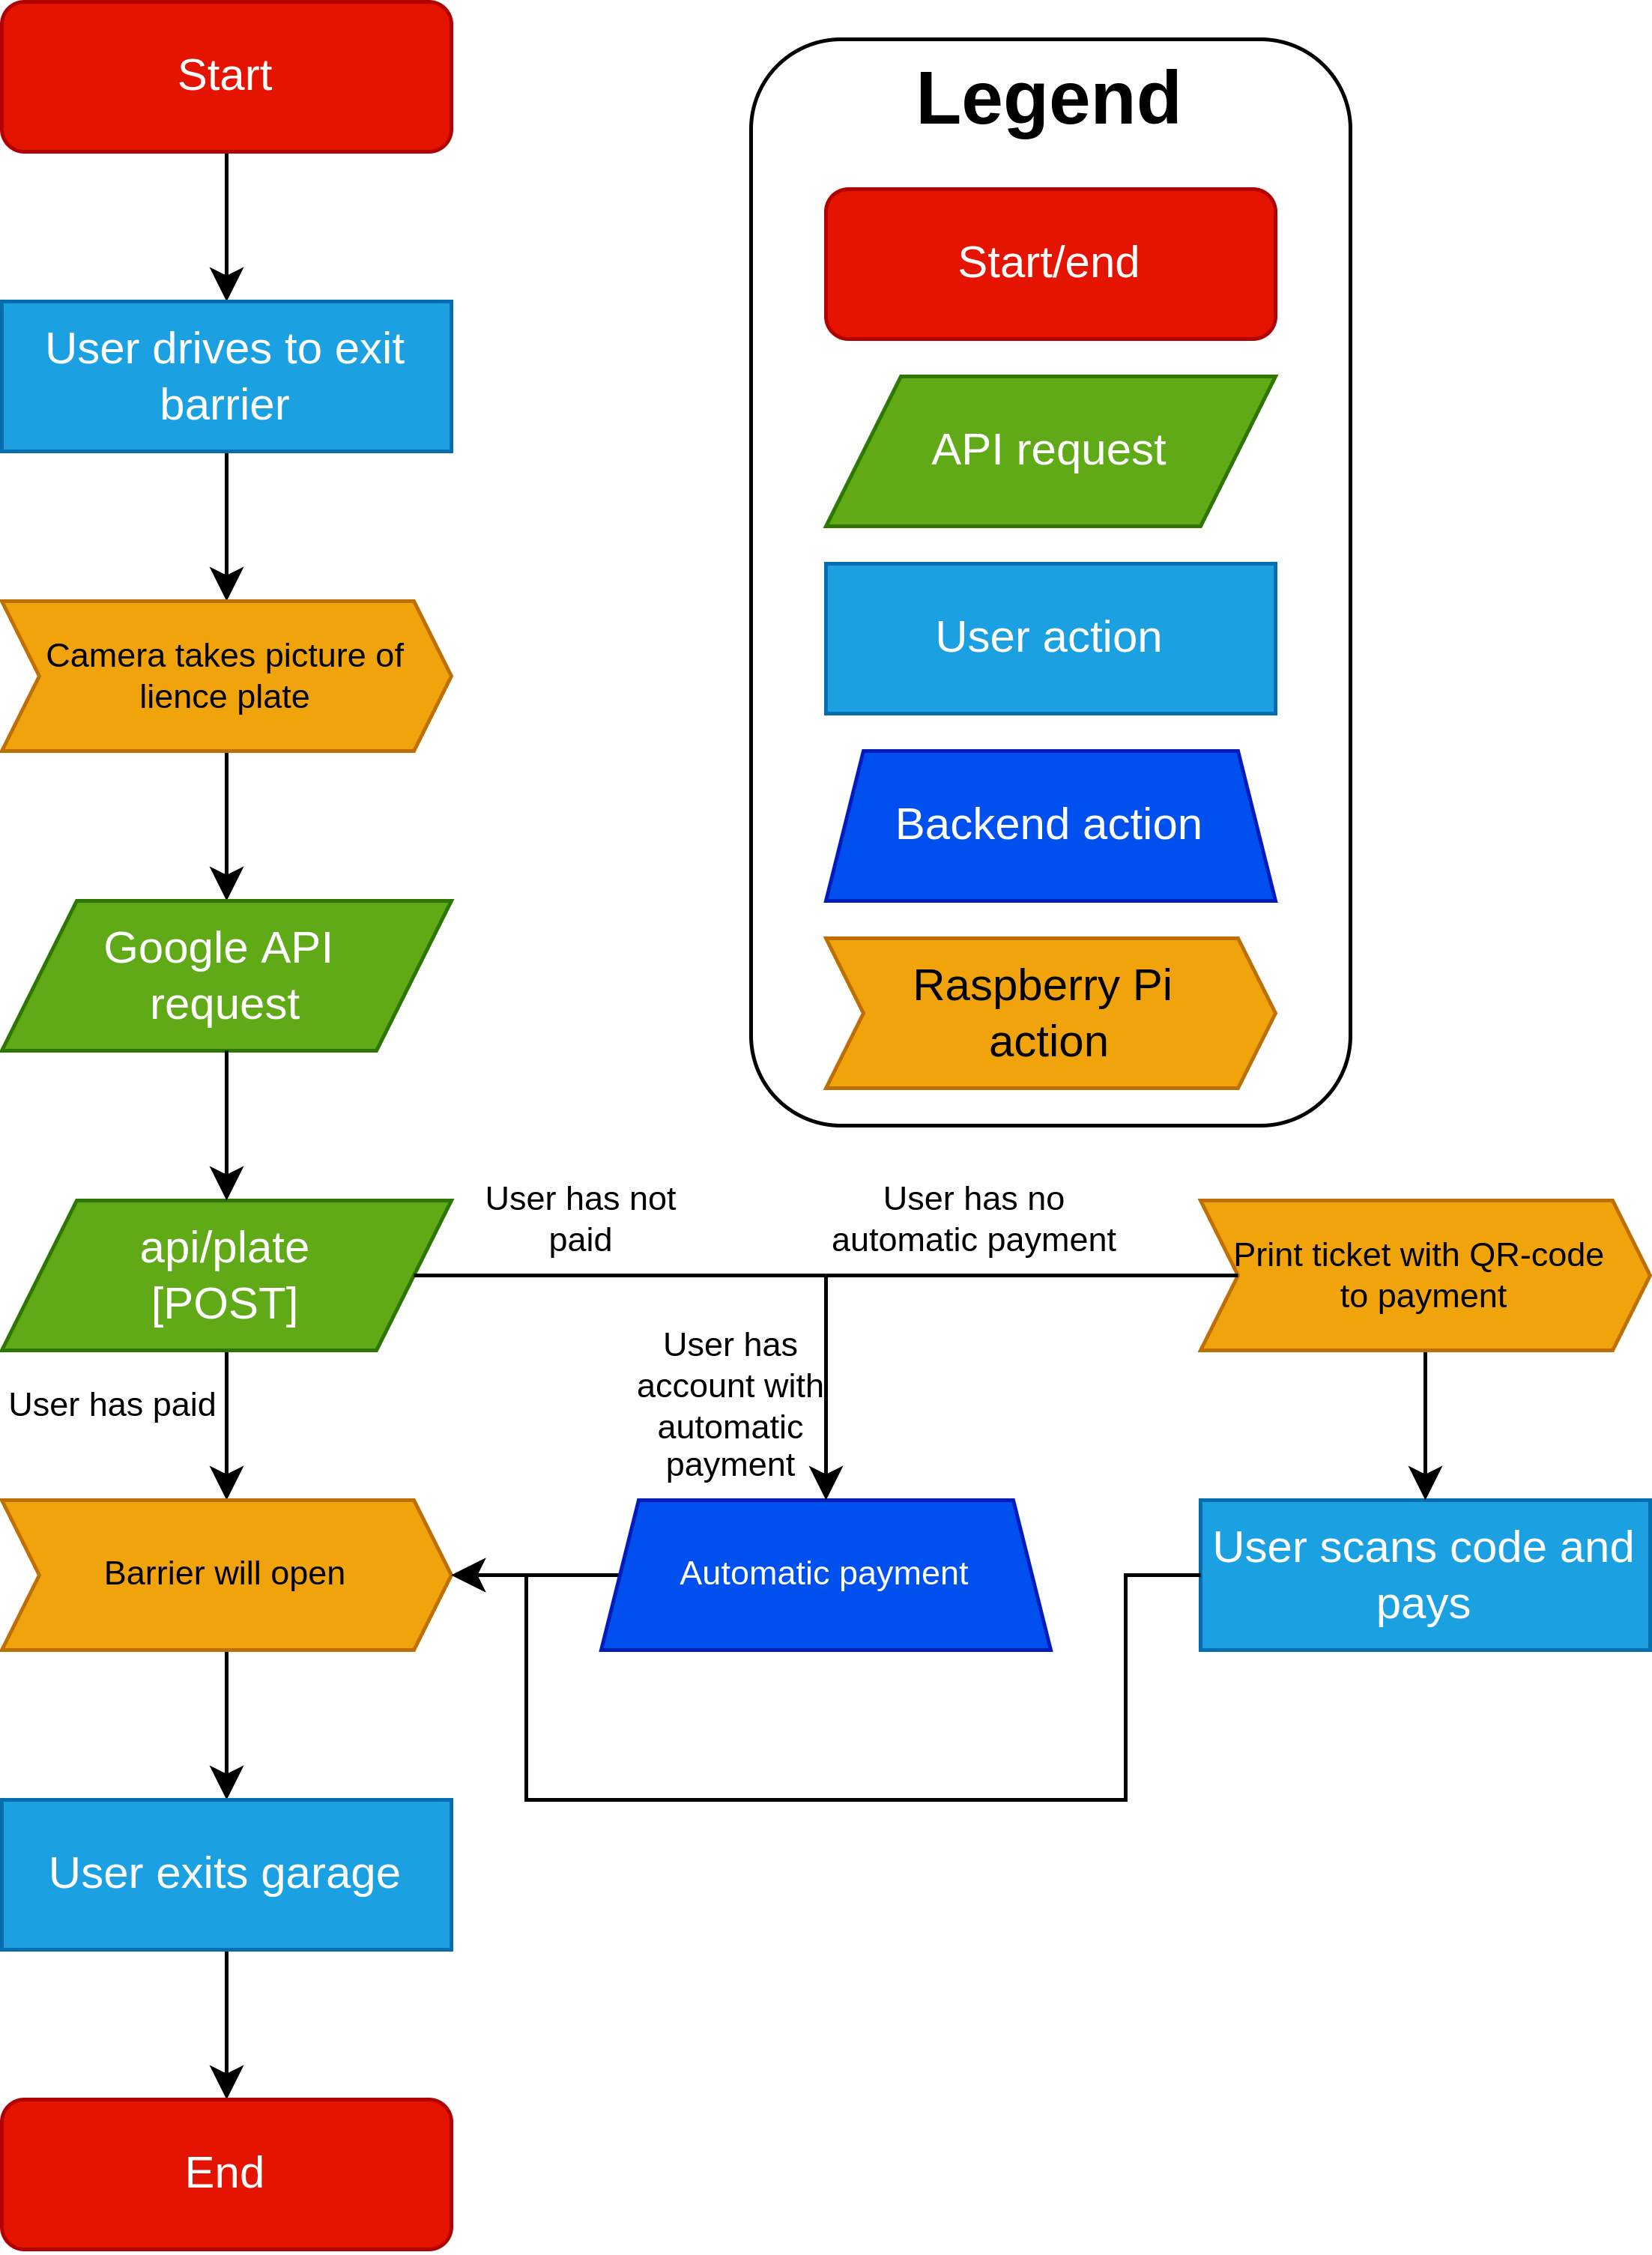
\includegraphics[width=8cm]{images/garage_exit.drawio.png}
    \caption{Flowchart of the exiting process of the garage in both hardware, software and user terms.}
    \label{fig:garage-exit}
\end{figure}

\section{Sequence diagrams}\label{app:sequence-diagrams}
\begin{figure}
    \centering
    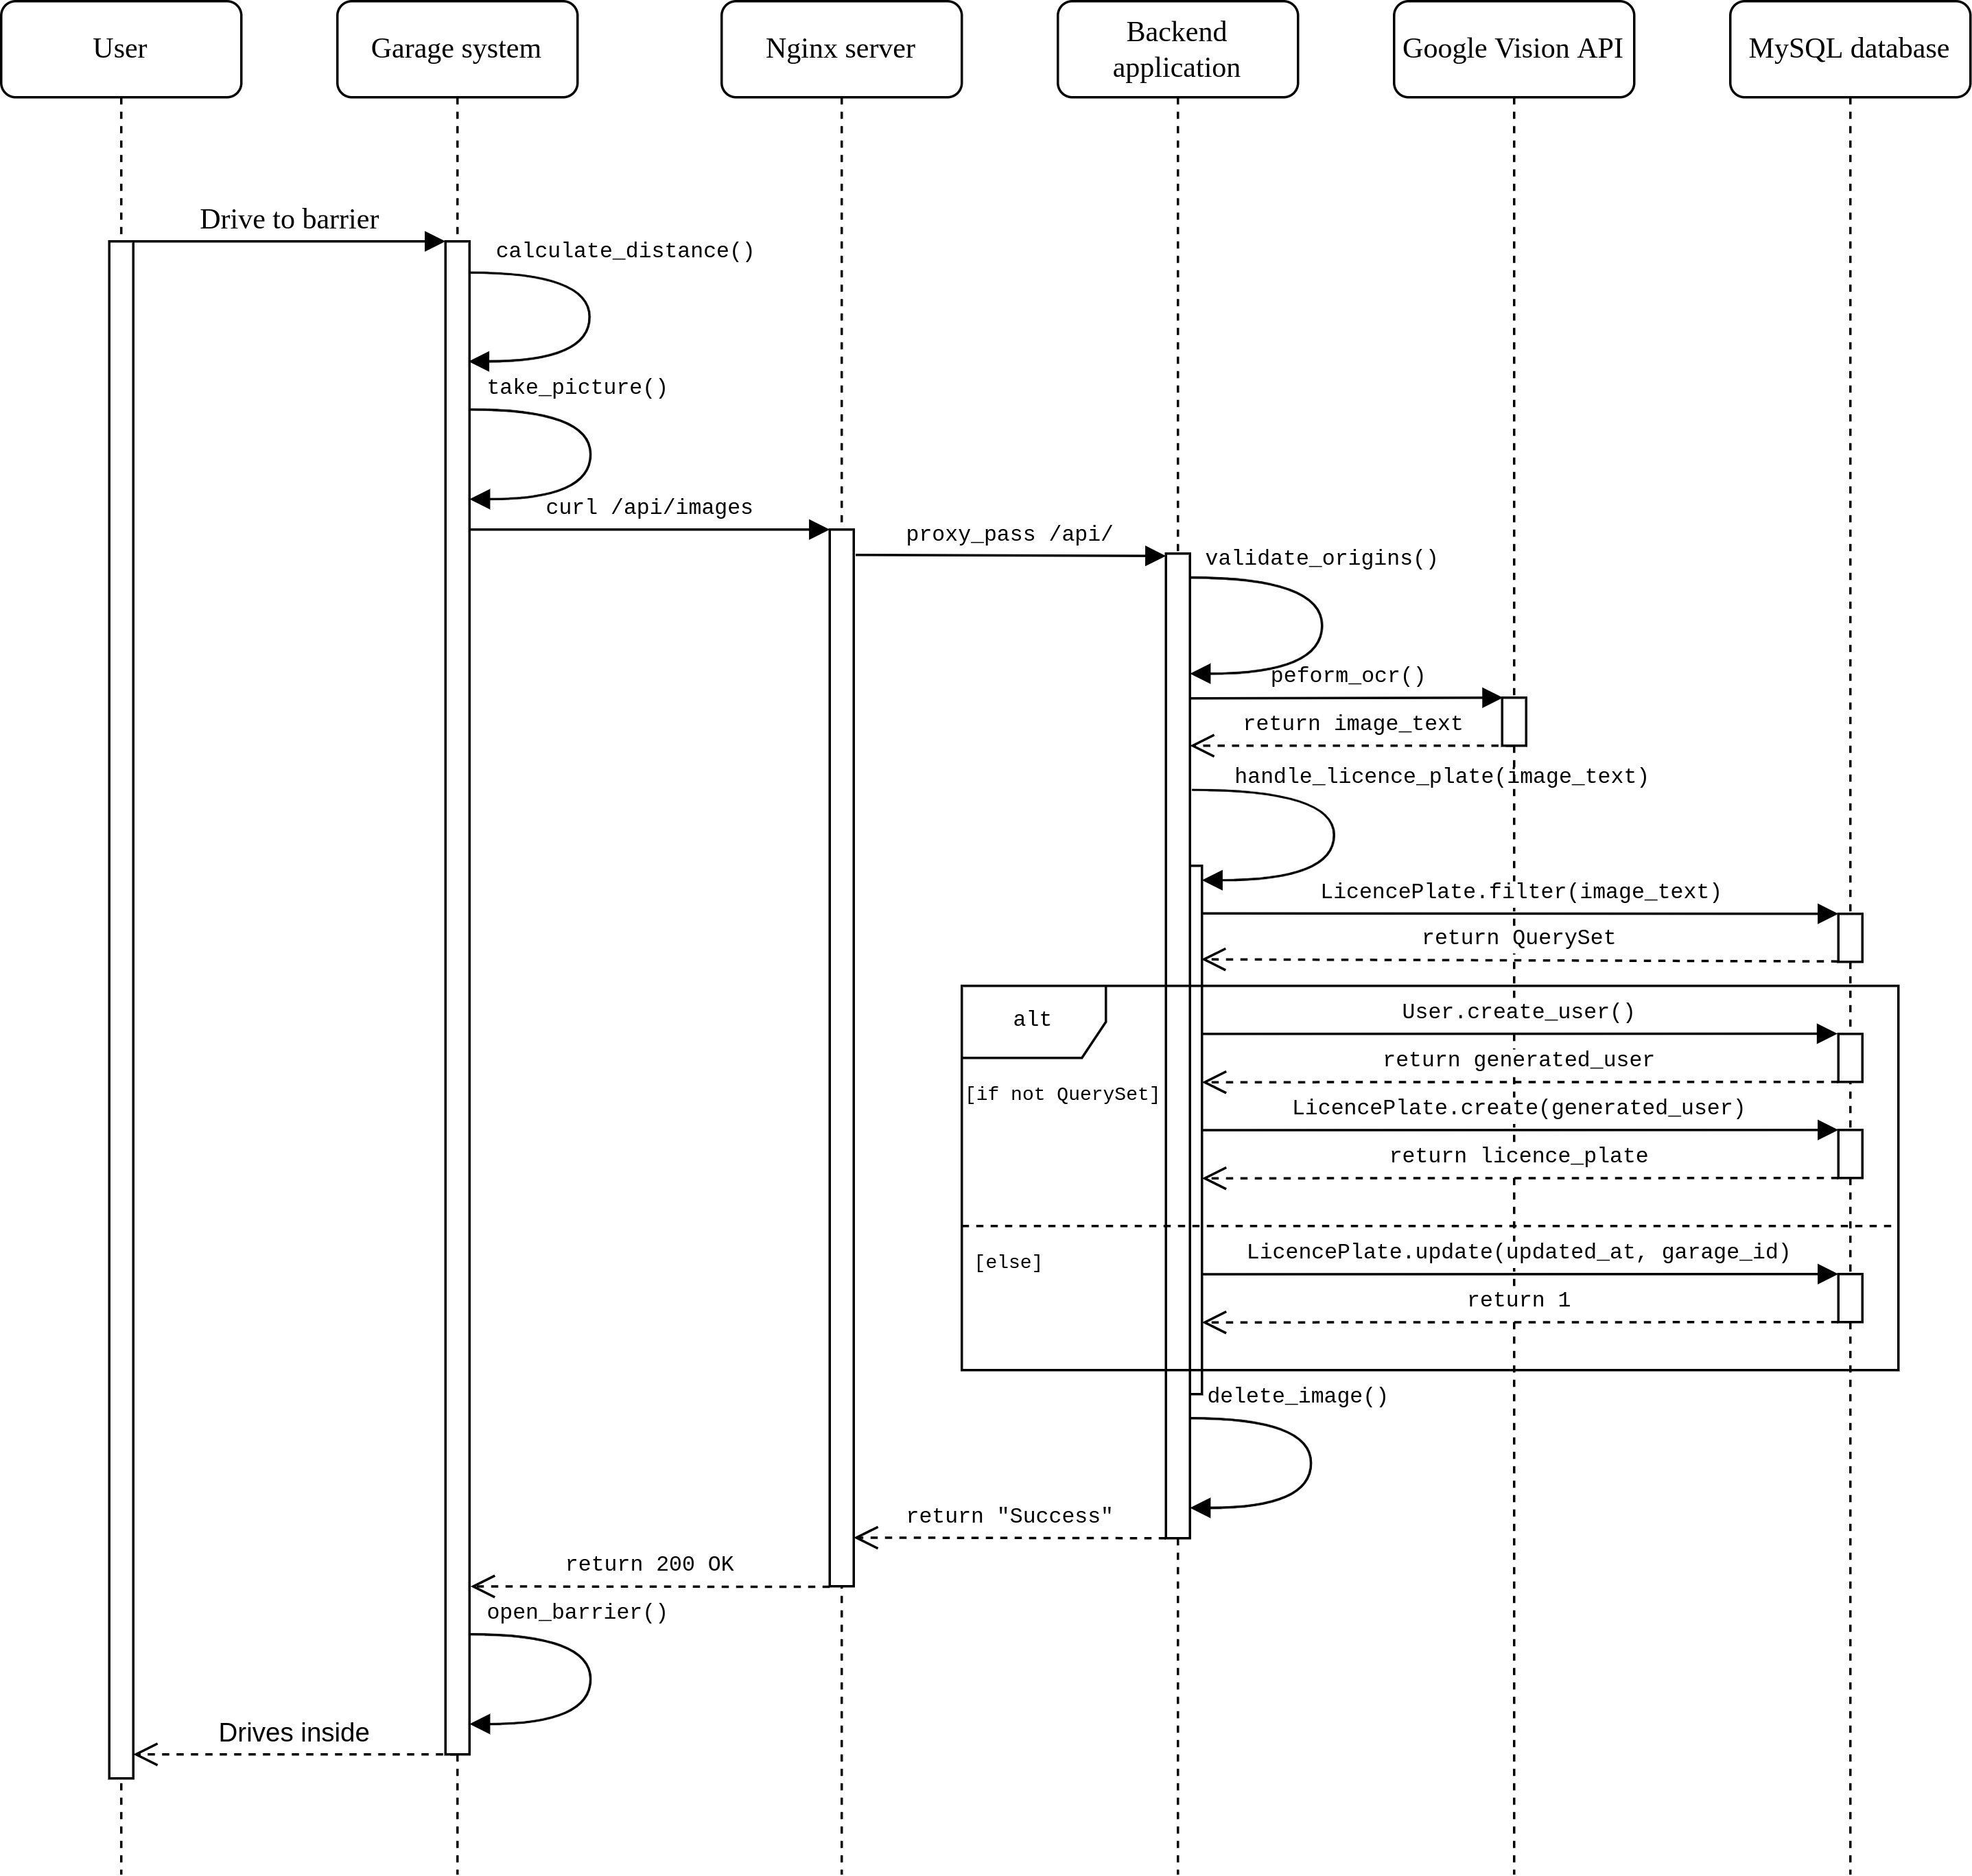
\includegraphics[width=16cm]{images/sequence_diagram_licence_plate.drawio.png}
    \caption{Sequence diagram of the licence plate registration in the local garage system.}
    \label{fig:sequence-diagram-licence-plate}
\end{figure}

\begin{figure}
    \centering
    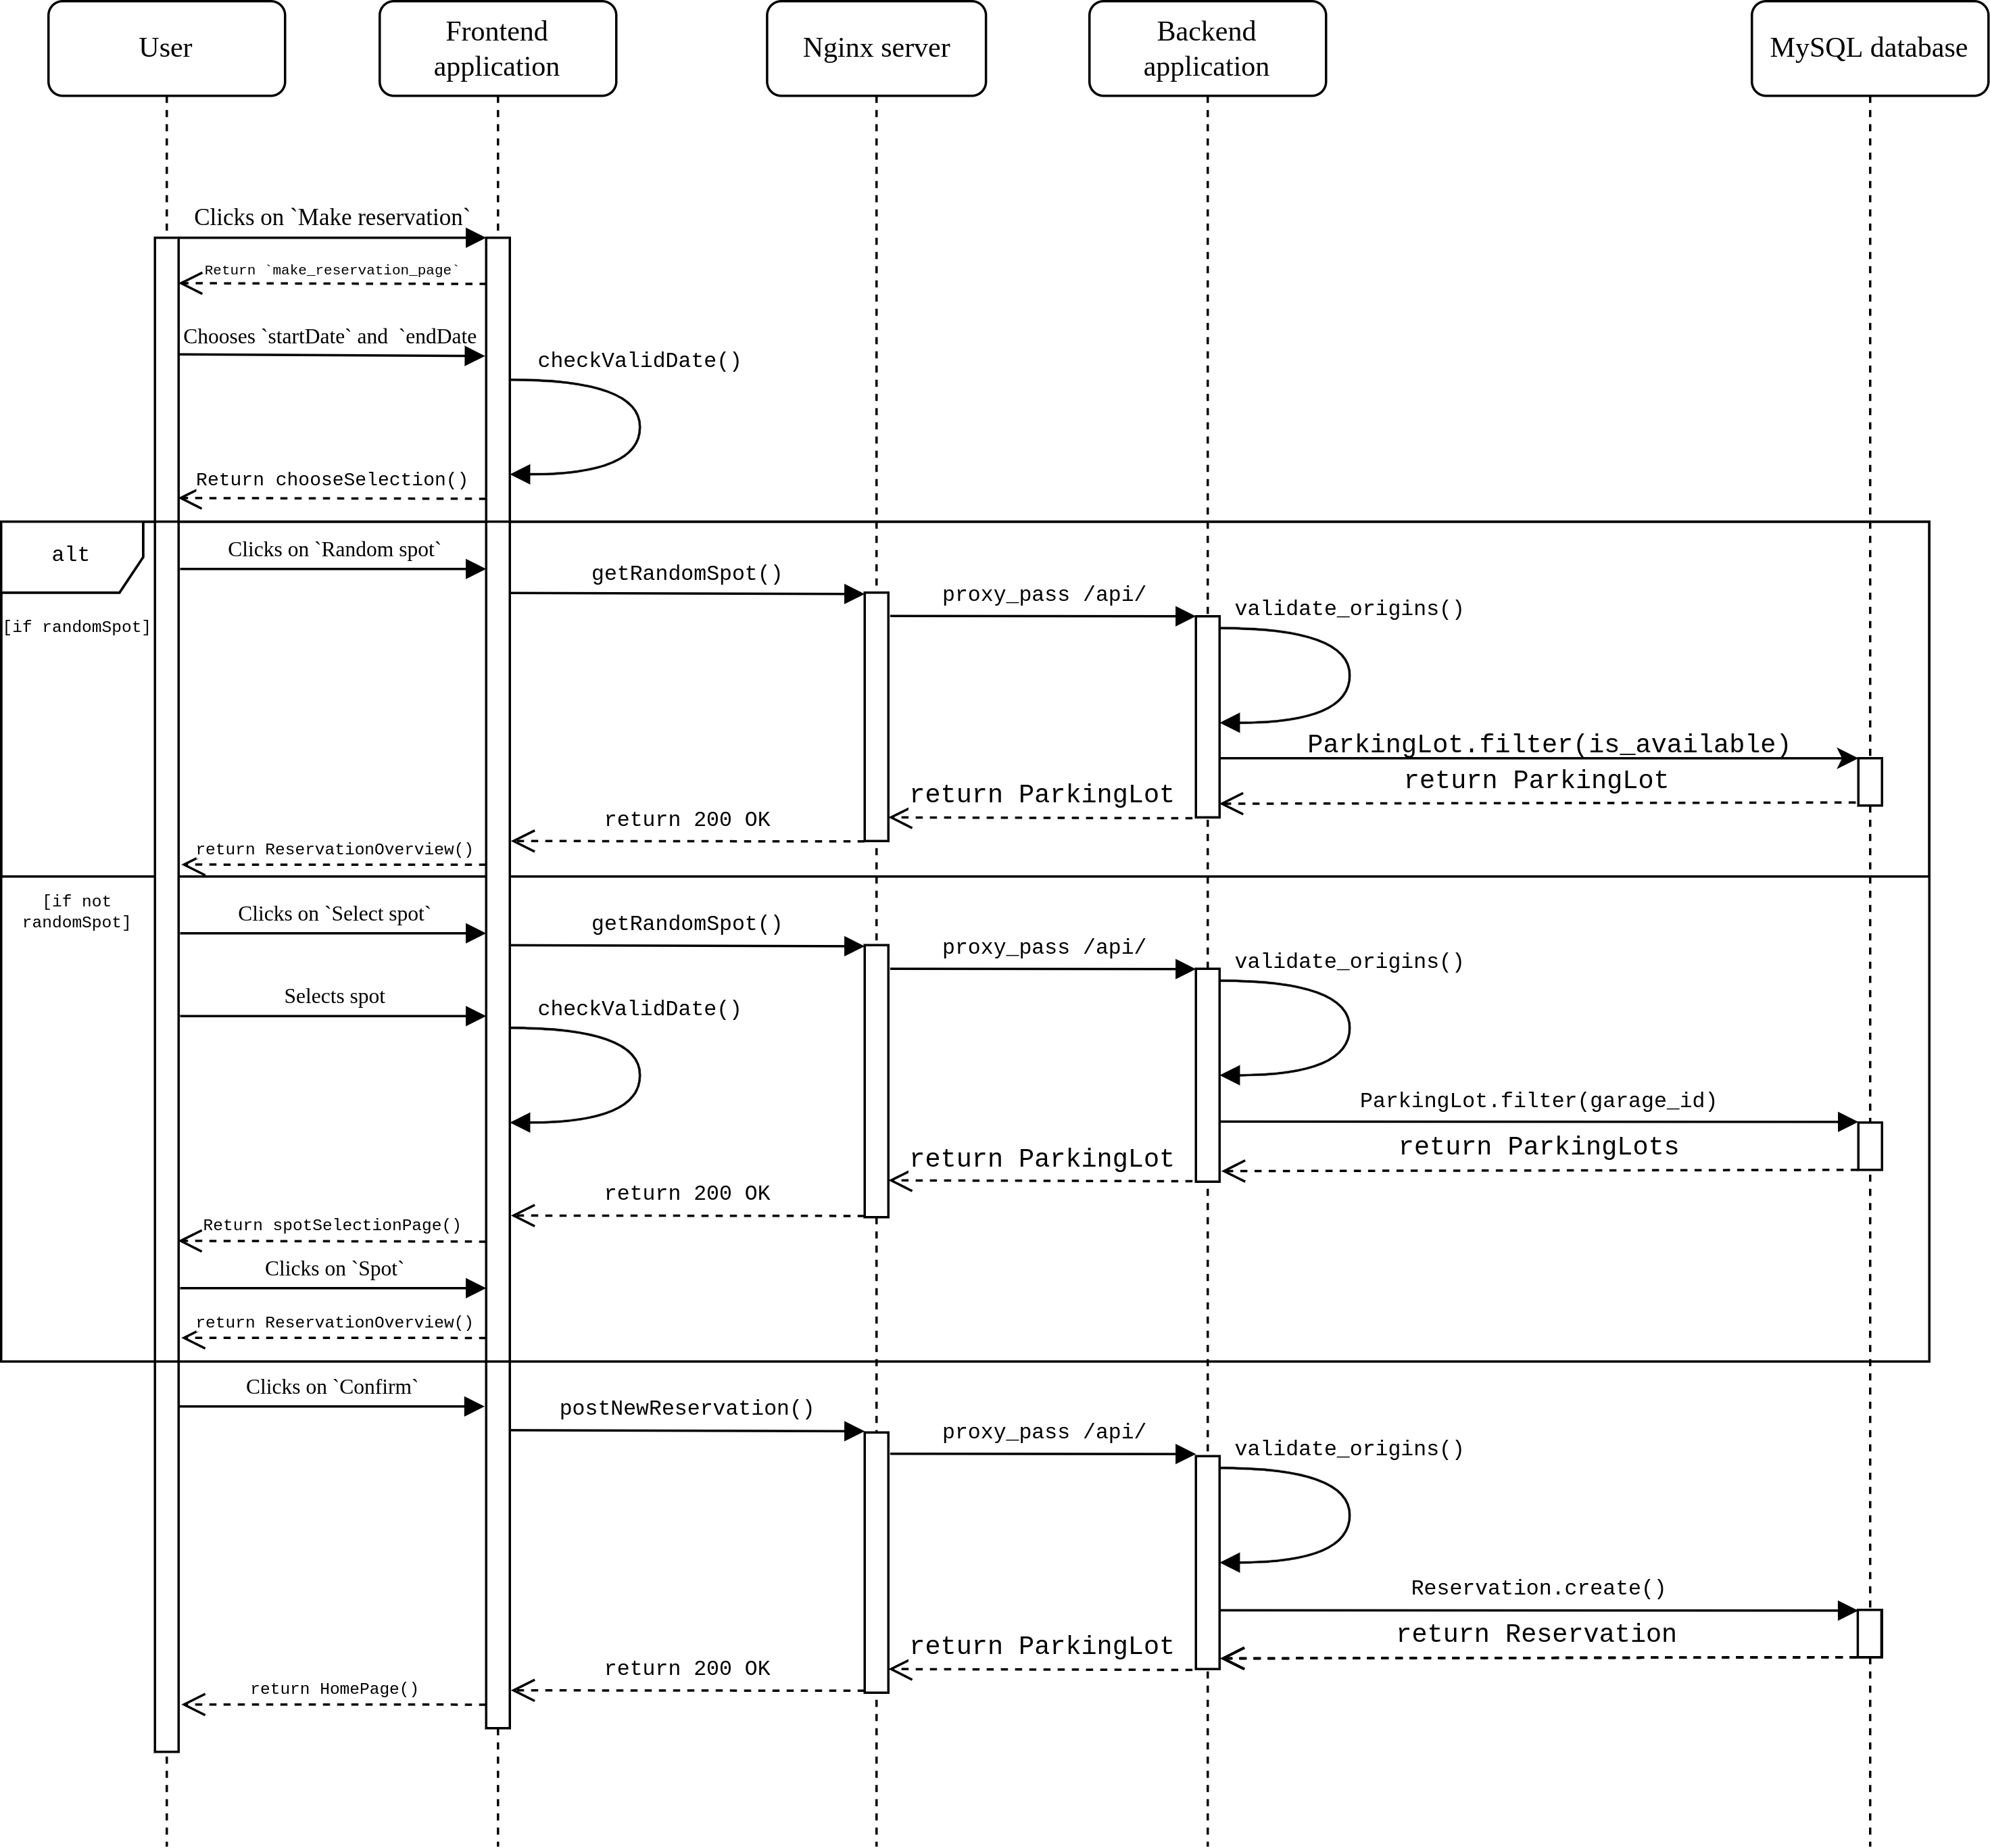
\includegraphics[width=16cm]{images/sequence_diagram_reservation.drawio.png}
    \caption{Sequence diagram of the reservation flow.}
    \label{fig:sequence-diagram-reservation}
\end{figure}

\end{appendices}
